\hyphenation{Nie-tzsche}
\chapter*{Sobre verdade e mentira\subtitulo{no sentido extramoral}}

\sectionitem
\noindent\textsc{Em algum remoto} recanto do universo, que se deságua fulgurantemente em
inumeráveis sistemas solares, havia uma vez um astro, no qual animais
astuciosos inventaram o conhecimento. Foi o minuto mais audacioso e
hipócrita da “história universal”: mas, no fim das contas, foi apenas
um minuto. Após alguns respiros da natureza, o astro congelou"-se, e
os astuciosos animais tiveram de morrer. Alguém poderia, desse modo,
inventar uma fábula e ainda assim não teria ilustrado suficientemente
bem quão lastimável, quão sombrio e efêmero, quão sem rumo e sem motivo
se destaca o intelecto humano no interior da natureza; houve
eternidades em que ele não estava presente; quando ele tiver passado
mais uma vez, nada terá ocorrido. Pois, para aquele intelecto, não há
nenhuma missão ulterior que conduzisse para além da vida humana. Ele é,
ao contrário, humano, sendo que apenas seu possuidor e gerador o toma
de maneira tão patética, como se os eixos do mundo girassem nele. 
Mas se pudéssemos pôr"-nos de acordo com o mosquito, aprenderíamos então
que ele também flutua pelo ar com esse \textit{pathos} e sente em si o
centro esvoaçante deste mundo. Na natureza, não há nada tão ignóbil e
insignificante que, com um pequeno sopro daquela força do conhecimento,
não inflasse, de súbito, como um saco; e assim como todo carregador de
peso quer ter seu admirador, o mais orgulhoso dos homens, o filósofo,
acredita ver por todos os lados os olhos do universo voltados
telescopicamente na direção de seu agir e pensar.\footnote{ Friedrich Nietzsche,
\textit{Über Wahrheit und Lüge im aussermoralischen Sinne}.
Em \textit{Sämtliche Werke. Kritische Studienausgabe},
Giorgio Colli e Mazzino Montinari, Berlim / Nova
York, Walter de Gruyter, 1999, pp.\,873--890.}

É curioso que isso seja levado a efeito pelo intelecto, precisamente
ele, que foi outorgado apenas como instrumento auxiliar aos mais
infelizes, frágeis e evanescentes dos seres, para conservá"-los um
minuto na existência; da qual, do contrário, sem essa outorga, eles
teriam todos os motivos para fugir tão rapidamente quanto o filho de
Lessing.\footnote{ Tido por Nietzsche como um “\textit{erudito ideal}”
(Cf.\,F.\,Nietzsche, Fragmento póstumo do inverno de 1869 e da primavera
de 1870, n° 2 [12]. Em \textit{Sämtliche Werke. Kritische
Studienausgabe}, Giorgio Colli e Mazzino Montinari, Berlim / Nova
York, Walter de Gruyter, 1999, vol.\,7, p.\,49), Gotthold Ephraim Lessing
(1729--1781) pondera, numa reveladora carta a Johann Joachim
Eschenburg, sobre a morte prematura de seu filho: “Minha alegria durou
pouco: perdi"-o com tamanha relutância, esse filho! Pois ele tinha
tanto entendimento! Tanto entendimento! Não pense que minhas poucas
horas de paternidade fizeram de mim uma besta de pai! Sei o que falo.
Não foi o entendimento que obrigou a puxá"-lo a férreo fórceps
para o mundo? Que tão cedo o levou a perceber sua desrazão? Não foi do
entendimento que ele se valeu na primeira oportunidade que teve para
abandoná"-lo novamente?” (Em G.\,E.\,Lessing, \textit{Kritik und
Dramaturgie. Ausgewählte Prosa}, Stuttgart, Reclam, 1957, p.\,84).}
Aquela audácia ligada ao conhecer e sentir, que se acomoda sobre os
olhos e sentidos dos homens qual uma névoa ofuscante, ilude"-os quanto
ao valor da existência, na medida em que traz em si a mais
envaidecedora das apreciações valorativas sobre o próprio conhecer. Seu
efeito mais universal é engano --- todavia, os efeitos mais particulares
também trazem consigo algo do mesmo caráter.

Como um meio para a conservação do indivíduo, o intelecto desenrola suas
principais forças na dissimulação; pois esta constitui o meio pelo qual
os indivíduos mais fracos, menos vigorosos, conservam"-se, como
aqueles aos quais é denegado empreender uma luta pela existência com
chifres e presas afiadas. No homem, essa arte da dissimulação atinge
seu cume: aqui, o engano, o adular, mentir e enganar, o falar pelas
costas, o representar, o viver em esplendor consentido, o mascaramento,
a convenção acobertadora, o fazer drama diante dos outros e de si
mesmo, numa palavra, o constante saracotear em torno da chama única da
vaidade, constitui a tal ponto a regra e a lei que quase nada é mais
incompreensível do que como pôde vir à luz entre os homens um legítimo
e puro impulso à verdade. Eles se acham profundamente imersos em
ilusões e imagens oníricas, seu olho desliza apenas ao redor da
superfície das coisas e vê “formas”, sua sensação não leva à verdade em
nenhum lugar, mas antes se satisfaz em receber estímulos e tocar, por
assim dizer, um teclado sobre o dorso das coisas. Para tanto, o homem
consente, à noite, e através de toda uma vida, ser enganado em sonho,
sem que seu sentimento moral jamais tentasse evitar isso: não obstante,
deve haver homens que, pela força de vontade, deixaram de roncar. O que
sabe o homem, de fato, sobre si mesmo! Seria ele sequer capaz, em algum
momento, de perceber"-se inteiramente, como se estivesse numa
iluminada cabine de vidro? Não se lhe emudece a natureza acerca de
todas as outras coisas, até mesmo acerca de seu corpo, para bani"-lo e
trancafiá"-lo numa consciência orgulhosa e enganadora, ao largo dos
movimentos intestinais, do veloz fluxo das correntes sanguíneas e das
complexas vibrações das fibras! Ela jogou fora a chave: e coitada da
desastrosa curiosidade que, através de uma fissura, fosse capaz de sair
uma vez sequer da câmara da consciência e olhar para baixo,
pressentindo que, na indiferença de seu não"-saber, o homem repousa
sobre o impiedoso, o voraz, o insaciável, o assassino, como se, em
sonhos, estivesse dependurado sobre as costas de um tigre. Então de
onde viria o impulso à verdade no mundo inteiro, nessa constelação?

Enquanto o indivíduo, num estado natural das coisas, quer preservar"-se
contra outros indivíduos, ele geralmente se vale do intelecto apenas
para a dissimulação: mas, porque o homem quer, ao mesmo tempo, existir
socialmente e em rebanho, por necessidade e tédio, ele necessita de um
acordo de paz e empenha"-se então para que a mais cruel \textit{bellum
omnium contra omnes} ao menos desapareça de seu mundo. Esse acordo de
paz traz consigo, porém, algo que parece ser o primeiro passo rumo à
obtenção daquele misterioso impulso à verdade. Agora, fixa"-se aquilo
que, doravante, deve ser “verdade”, quer dizer, descobre"-se uma
designação uniformemente válida e impositiva das coisas, sendo que a
legislação da linguagem fornece também as primeiras leis da verdade:
pois aparece, aqui, pela primeira vez, o contraste entre verdade e
mentira; o mentiroso serve"-se das designações válidas, as palavras,
para fazer o imaginário surgir como efetivo; ele diz, por exemplo,
“sou rico”, quando para seu estado justamente “pobre” seria a
designação mais acertada. Ele abusa das convenções consolidadas por
meio de trocas arbitrárias ou inversões dos nomes, inclusive. Se 
faz isso de uma maneira individualista e ainda por cima nociva,
então a sociedade não confiará mais nele e, com isso, tratará de
excluí"-lo. Nisso, os homens não evitam tanto ser ludibriados
quanto lesados pelo engano. Mesmo nesse nível, o que eles odeiam
fundamentalmente não é o engano, mas as consequências ruins, hostis, de
certos gêneros de enganos. Num sentido semelhantemente limitado, o homem
também quer apenas a verdade. Ele quer as consequências agradáveis da
verdade, que conservam a vida; frente ao puro conhecimento sem
consequências ele é indiferente, frente às verdades possivelmente
prejudiciais e destruidoras ele se indispõe com hostilidade, inclusive.
E mais até: como ficam aquelas convenções da linguagem? São talvez
produtos do conhecimento, do sentido de verdade: as designações e as
coisas se recobrem? Então a linguagem é a expressão adequada de todas
as realidades?
Apenas por esquecimento pode o homem alguma vez chegar a imaginar que
detém uma verdade no grau ora mencionado. Se ele não espera
contentar"-se com a verdade sob a forma da tautologia, isto é, com
conchas vazias, então irá permutar eternamente ilusões por verdades. O
que é uma palavra? A reprodução de um estímulo nervoso em sons. Mas
deduzir do estímulo nervoso uma causa fora de nós já é o resultado de
uma aplicação falsa e injustificada do princípio de razão. Como
poderíamos, caso tão"-somente a verdade fosse decisiva na gênese da
linguagem, caso apenas o ponto de vista da certeza fosse algo decisório
nas designações, como poderíamos nós, não obstante, dizer: a pedra é
dura; como se esse “dura” ainda nos fosse conhecido de alguma outra
maneira e não só como um estímulo totalmente subjetivo! Seccionamos as
coisas de acordo com gêneros, designamos a árvore como feminina e o
vegetal como masculino: mas que transposições arbitrárias! Quão longe
voamos para além do cânone da certeza! Falamos sobre uma serpente: a
designação não tange senão ao ato de serpentear e, portanto, poderia
servir também ao verme. Mas que demarcações arbitrárias, que
preferências unilaterais, ora por esta, ora por aquela propriedade de
uma dada coisa! Dispostas lado a lado, as diferentes línguas mostram
que, nas palavras, o que conta nunca é a verdade, jamais uma expressão
adequada: pois, do contrário, não haveria tantas línguas. A “coisa em
si” (ela seria precisamente a pura verdade sem quaisquer consequências)
também é, para o criador da linguagem, algo totalmente inapreensível e
pelo qual nem de longe vale a pena esforçar"-se. Ele designa apenas as
relações das coisas com os homens e, para expressá"-las, serve"-se da
ajuda das mais ousadas metáforas. De antemão, um estímulo nervoso
transposto em uma imagem! Primeira metáfora. A imagem, por seu turno,
remodelada num som! Segunda metáfora. E, a cada vez, um completo
sobressalto de esferas em direção a uma outra totalmente diferente e
nova. Pode"-se conceber um homem que seja completamente surdo e que
jamais tenha tido uma sensação do som e da música: da mesma forma que
este, um tanto espantado com as figuras sonoras de Chladni sobre a
areia,\footnote{ O texto faz menção ao experimento levado a cabo pelo
físico alemão Ernst Chladni (1756--1827) que se destina a
verificar a ocorrência de certas formas vibratórias e que convém, aqui,
explicitar. Basicamente, trata"-se de cobrir a superfície de uma placa
circular de madeira, vidro ou metal, com leves partículas de areia --- em
realidade, cortiça em pó para, com o auxílio de um arco de violino,
provocar vibrações em lugares específicos na borda do disco assim
disposto. Em consequência das vibrações, as partículas da placa
terminam por se dividir em diversas seções, movimentando"-se aqui e
acolá, para cima e para baixo, formando traços limítrofes e linhas
nodais entre as áreas mais agitadas e as zonas com menor intensidade
vibrátil. Ao longo de tal processo, as partículas polvilhadas tendem a
espalhar"-se em meio às extensões mais vibrantes e acumular"-se lá,
onde a vibração é menor, de sorte que, de acordo com a forma do disco e
conforme o local em que nele é provocado o movimento vibratório,
diferentes figuras sonoras vêm à superfície. Aqui o melhor
mesmo é recorrer às palavras do próprio físico alemão. Em sua principal
obra, \textit{A acústica}, ele diz: “As placas podem ser de vidro ou de
um metal bastante sonoro [\ldots{}] Pode"-se servir, inclusive, de placas
de madeira, mas, nesse caso, as figuras não serão regulares, já que a
elasticidade não é a mesma nos diferentes sentidos. Normalmente,
sirvo"-me de placas de vidro, já que é possível encontrá"-las
facilmente sob a mesma espessura e porque sua transparência permite
enxergar os locais nos quais são tocadas, com os dedos, por debaixo”.
(Ernst Chladni, \textit{Die Akustik}, Leipzig,
Breitkopf u.\,Härtel, 1802, p.\,118--19). Mais adiante, especificamente
sobre as placas circulares, ele esclarece: “No que tange aos tipos de
vibração de uma placa circular, as linhas nodais são ou diametrais ou
circulares [\ldots{}] Exprimirei o número de linhas nodais da mesma forma
que os das placas retangulares, posicionando o número atinente às
linhas nodais nas direções diametrais antes do traço que separa os dois
números por mim indicados, e, depois do traço, o número de linhas
nodais paralelas à borda, sendo que estes últimos serão escritos em
algarismos romanos. Assim, por exemplo, 2/0 irá indicar o tipo de
vibração no qual não há senão duas linhas diametrais; 0/1 aquele que
não apresenta senão uma linha circular [\ldots{}] 2/0 em que duas linhas
diametrais se cruzam no centro [figura 99] é, dentre todas as
figuras possíveis, aquela equivale ao som mais grave''.\\*
\mbox{}\hfil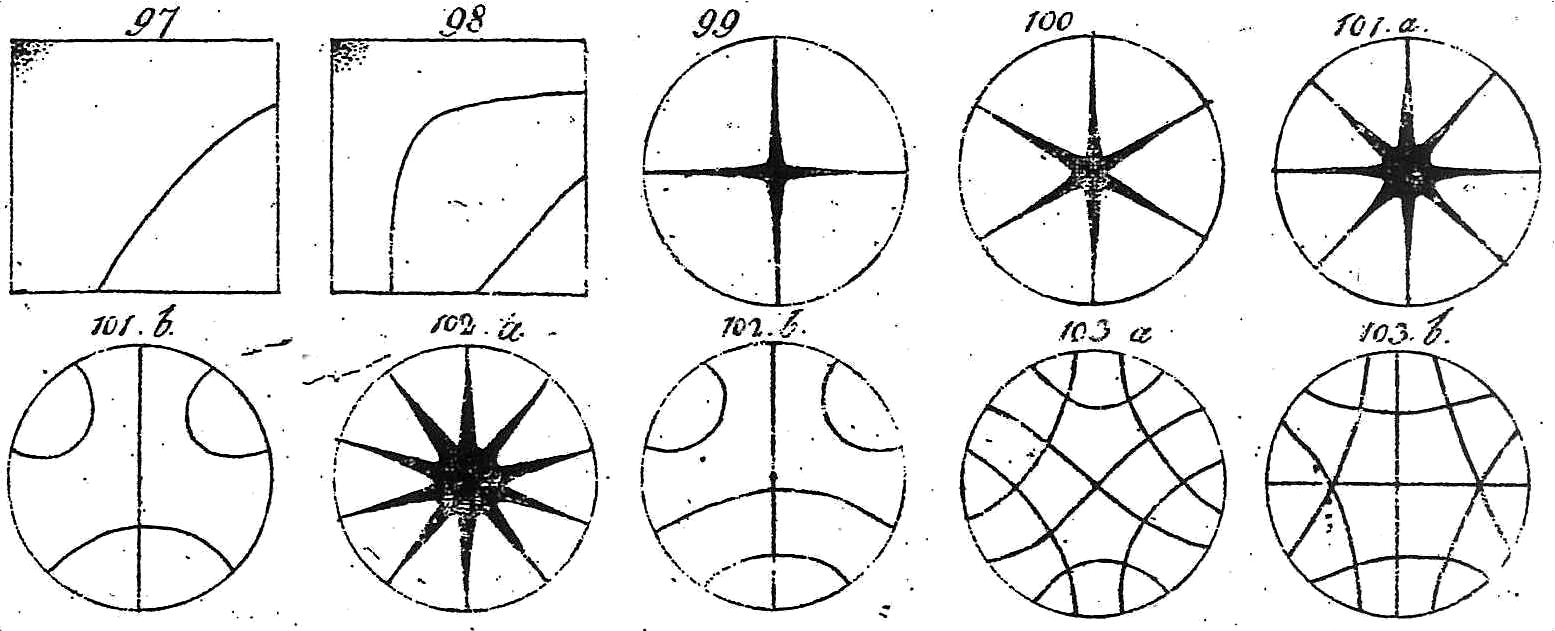
\includegraphics[width=7cm]{imagem.png}\hfil\\*
\mbox{}\hfill(\textit{Ibid}.\,p.\,156--157.)}
encontra suas causas na vibração
das cordas e jurará que agora não pode mais ignorar aquilo que os
homens chamam de som, assim também sucede a todos nós com a
linguagem. Acreditamos saber algo acerca das próprias coisas, quando
falamos de árvores, cores, neve e flores, mas, com isso, nada possuímos
senão metáforas das coisas, que não correspondem, em absoluto, às
essencialidades originais. Tal como o som sob a forma de figura de
areia, assim se destaca o enigmático ``\textsc{x}'' da coisa em si, uma vez como
estímulo nervoso, em seguida como imagem, e, por fim, como
som.\footnote{ As figuras de Chladni são oportunas a Nietzsche, porque
servem para indicar, a partir do âmbito sonoro, a impossibilidade de
expressar adequadamente a “verdadeira” realidade do mundo. Assim como
tais figuras se incumbem de editar cópias dos sons noutro meio --- na
areia, no caso, assim também se relacionariam as palavras com as
coisas, a saber, a partir da transposição de um estímulo nervoso em
imagem e, depois, em som. O homem, inflexível em relação ao enigmático
“\textsc{x}” por detrás do que fala e escuta, contemplaria em vão os desenhos
sonoros sem neles descerrar qualquer passagem ao legítimo “ser” das
coisas. Afinal, como dirá Nietzsche alhures: “Não podemos pensar as coisas
tais como elas são, pois não deveríamos justamente pensá"-las. Tudo
permanece assim, tal como é: isto é, todas as qualidades revelam uma
matéria indefinida e absoluta. A relação aqui se dá como aquela que
as figuras sonoras de Chladni estabelecem com as vibrações” (F.\,Nietzsche,
Fragmento póstumo do verão de 1872 e início de 1873, n° 19 [140].
Em \textit{Sämtliche Werke. Kritische Studienausgabe}, Giorgio
Colli e Mazzino Montinari, Berlim / Nova York, Walter de Gruyter, 1999,
vol.\,7, p.\,464).} De qualquer modo, o surgimento da linguagem não
procede, pois, logicamente, sendo que o inteiro material no qual e com
o qual o homem da verdade, o pesquisador, o filósofo, mais tarde
trabalha e edifica, tem sua origem, se não em alguma nebulosa
cucolândia, em todo caso não na essência das coisas.

Ponderemos ainda, em especial, sobre a formação dos conceitos: toda palavra
torna"-se de imediato um conceito à medida que não deve servir, a
título de recordação, para a vivência primordial completamente singular
e individualizada à qual deve seu surgimento, senão que, ao mesmo
tempo, deve coadunar"-se a inumeráveis casos, mais ou menos
semelhantes, isto é, nunca iguais quando tomados à risca, a casos
nitidamente desiguais, portanto. Todo conceito surge pela igualação do
não"-igual. Tão certo como uma folha nunca é totalmente igual a uma
outra, é certo ainda que o conceito de folha é formado por meio de uma
arbitrária abstração dessas diferenças individuais, por um
esquecer"-se do diferenciável, despertando então a representação, como se
na natureza, além das folhas, houvesse algo que fosse “folha”, tal como uma
forma primordial de acordo com a qual todas as folhas fossem tecidas,
desenhadas, contornadas, coloridas, encrespadas e pintadas, mas por
mãos ineptas, de sorte que nenhum exemplar resultasse correto e
confiável como cópia autêntica da forma primordial. Denominamos um
homem honesto; perguntamos então: por que motivo ele agiu hoje de modo
tão honesto? Nossa resposta costuma ser a seguinte: em função de sua
honestidade. A honestidade! Uma vez mais, isso significa: a folha é a
causa das folhas. Nada sabemos, por certo, a respeito de uma qualidade
essencial que se chamasse honestidade, mas, antes do mais, de
inúmeras ações individualizadas e, por conseguinte, desiguais, que
igualamos por omissão do desigual e passamos a designar, desta feita,
como ações honestas; a partir delas formulamos, finalmente, uma
\textit{qualitas occulta} com o nome: honestidade.

A inobservância do individual e efetivo nos fornece o conceito, bem como
a forma, ao passo que a natureza desconhece quaisquer formas e
conceitos, e, portanto, também quaisquer gêneros, mas tão"-somente um
``\textsc{x}'' que nos é inacessível e indefinível. Pois até mesmo nossa oposição
entre indivíduo e gênero é antropomórfica, e não advém da essência das
coisas, ainda que não arrisquemos dizer que ela não lhe corresponde:
isso seria, efetivamente, uma asserção dogmática e, como tal, tão
indemonstrável quanto o seu contrário.

O que é, pois, a verdade? Um exército móvel de metáforas, metonímias,
antropomorfismos, numa palavra, uma soma de relações humanas que foram
realçadas poética e retoricamente, transpostas e adornadas, e que, após
uma longa utilização, parecem a um povo consolidadas, canônicas e
obrigatórias: as verdades são ilusões das quais se esqueceu que elas
assim o são, metáforas que se tornaram desgastadas e sem força
sensível, moedas que perderam seu troquel e agora são levadas em conta
apenas como metal, e não mais como moedas. Ainda não sabemos donde provém o
impulso à verdade: pois, até agora, ouvimos falar apenas da obrigação
de ser veraz, que a sociedade, para existir, institui, isto é, de
utilizar as metáforas habituais; portanto, dito moralmente: da
obrigação de mentir conforme uma convenção consolidada, mentir em
rebanho num estilo a todos obrigatório. O homem decerto se esquece que
é assim que as coisas se lhe apresentam; ele mente, pois, da maneira
indicada, inconscientemente e conforme hábitos seculares --- e
precisamente \textit{por meio dessa inconsciência}, justamente mediante
esse esquecer"-se, atinge o sentimento da verdade. No sentimento de
estar obrigado a indicar uma coisa como vermelha, outra como fria e
uma terceira como muda, sobrevém uma emoção moral 
atinente à verdade: a
partir da contraposição ao mentiroso, àquele em quem ninguém confia e
que todos excluem, o homem demonstra para si o que há de venerável,
confiável e útil na verdade. Como ser \textit{racional}, põe seu 
agir sob o império das abstrações: já não tolera mais ser arrastado
por impressões repentinas, pelas intuições, sendo que universaliza,
antes, todas essas impressões em conceitos mais desbotados e frios,
para neles atrelar o veículo de seu viver e agir. Tudo aquilo que
sobreleva o homem ao animal depende dessa capacidade de volatilizar as
metáforas intuitivas num esquema, de dissolver uma imagem num conceito,
portanto; no âmbito daqueles esquemas, torna"-se possível algo que
nunca poderia ser alcançado sob a égide das primeiras impressões
intuitivas: erigir uma ordenação piramidal segundo castas e gradações,
criar um novo mundo de leis, privilégios, subordinações, delimitações,
que agora faz frente ao outro mundo intuitivo das primeiras impressões
como o mais consolidado, universal, conhecido, humano e, em virtude
disso, como o mundo regulador e imperativo. Enquanto cada metáfora
intuitiva é individual e desprovida de seu correlato, e, por isso, sabe
sempre eludir a todo rubricar, o grande edifício dos conceitos exibe a
inflexível regularidade de um columbário romano e 
exala na lógica aquela
dureza e frieza que são próprias à matemática. Aquele que é baforado
por essa frieza mal acreditará que mesmo o conceito, ossificado e
octogonal como um dado e tão rolante como este, permanece tão"-somente
o \textit{resíduo de uma metáfora}, sendo que a ilusão da transposição
artística de um estímulo nervoso em imagens, se não é a mãe, é ao menos
a avó de todo conceito. Mas, no interior desse jogo de dados dos
conceitos, denomina"-se “verdade” a utilização de cada dado tal como
ele é designado; contar seus pontos com acuidade, formar rubricas
corretas e jamais atentar contra a ordenação de castas, bem como contra
a sequência das classes hierarquicamente organizadas. Tal como os
romanos e etruscos dissecavam o céu através de firmes linhas
matemáticas e relegavam um deus num espaço assim demarcado, como num
templo, assim cada povo tem sobre si um equivalente céu conceitual
matematicamente dividido e, sob a exigência da verdade, agora entende
que cada deus conceitual deve ser buscado apenas em \textit{sua} esfera.
Aqui, cabe muito bem admirar o homem como um formidável gênio da
construção, capaz de erguer sobre fundamentos instáveis e como que
sobre água corrente um domo de conceitos infinitamente complicado; por
certo, a fim de manter"-se firmemente em pé sobre tais fundamentos,
cumpre ser uma construção como que feita com teias de aranha,
suficientemente delicada que possa ser levada pelas ondas e firme o
bastante para não ser despedaçada pelo sopro do vento. Como gênio da
construção, o homem eleva"-se muito acima da abelha na seguinte
medida: esta última constrói a partir da cera, que ela recolhe da
natureza, ao passo que o primeiro a partir da matéria muito mais
delicada dos conceitos, que precisa fabricar a partir de si mesmo. Aqui,
cumpre admirá"-lo muito, mas não somente por causa de seu impulso à
verdade, ao conhecimento puro das coisas. Quando alguém esconde algo
detrás de um arbusto, volta a procurá"-lo justamente lá onde o
escondeu e além de tudo o encontra, não há muito do que se vangloriar
nesse procurar e encontrar: é assim que se dá com o procurar e
encontrar da “verdade” no interior do domínio da razão. Se crio a
definição de mamífero e, aí então, após inspecionar um camelo, declaro:
veja, eis um mamífero, com isso, uma verdade decerto é trazida à plena
luz, mas ela possui um valor limitado, digo, ela é antropomórfica de
fio a pavio e não contém um único ponto sequer que fosse “verdadeiro em
si”, efetivo e universalmente válido, deixando de lado o homem. Em princípio, 
o pesquisador dessas verdades procura apenas a metamorfose do
mundo nos homens; esforça"-se por uma compreensão do mundo visto como uma coisa
própria ao homem e, na melhor das hipóteses, granjeia para si o
sentimento de uma assimilação. À semelhança do astrólogo que observa as
estrelas a serviço dos homens e em conformidade com sua felicidade e
sofrimento, assim também um tal pesquisador observa o mundo inteiro 
como conectado ao homem, como o ressoar infinitamente fragmentado de um
som primordial, do homem, como a cópia reduplicada de uma imagem
primordial, do homem. Eis seu procedimento: ter o homem por medida de
todas as coisas, algo que ele faz, porém, partindo do erro de acreditar
que teria tais coisas como objetos puros diante de si. Ele se esquece,
pois, das metáforas intuitivas originais tais como são, metáforas,
e as toma pelas próprias coisas.

Somente pelo esquecimento desse mundo metafórico primitivo, apenas pelo
enrijecimento e petrificação de uma massa imagética que, qual um
líquido fervente, desaguava originalmente em torrentes a partir da
capacidade primitiva da fantasia humana, tão"-somente pela crença imbatível
de que \textit{este} sol, \textit{esta} janela, esta mesa são uma
verdade em si, em suma, apenas por que o homem se esquece
enquanto sujeito e, com efeito, enquanto sujeito \textit{artisticamente
criador}, ele vive com certa tranquilidade, com alguma segurança e
consequência; se pudesse sair apenas por um instante das redomas
aprisionadoras dessa crença, então sua “autoconsciência” desapareceria
de imediato. Exige"-lhe esforço, inclusive, admitir para si mesmo o fato
de que o inseto ou o pássaro percebem um mundo totalmente diferente
daquele percebido pelo homem, sendo que a pergunta por qual das duas
percepções de mundo é a mais correta não possui qualquer sentido, haja
vista que, para respondê"-la, a questão teria de ser previamente
medida com o critério atinente à \textit{percepção correta}, isto é, de
acordo com um critério que \textit{não está à disposição}. A mim me
parece, em todo caso, que a percepção correta --- que significaria a
expressão adequada de um objeto no sujeito --- é uma contraditória
absurdidade: pois, entre duas esferas absolutamente diferentes tais
como entre sujeito e objeto não vigora nenhuma causalidade, nenhuma
exatidão, nenhuma expressão, mas, acima de tudo, uma relação
\textit{estética}, digo, uma transposição sugestiva, uma tradução
balbuciante para uma língua totalmente estranha. Algo que requer, de
qualquer modo, uma esfera intermediária manifestamente poética e
inventiva, bem como uma força mediadora. A palavra aparência contém
muitas tentações, daí eu evitá"-la sempre que possível: pois não é
verdade que a essência das coisas aparece no mundo empírico. Um pintor
cujas mãos lhe faltassem e quisesse, ainda assim, expressar pelo canto
a imagem por ele visionada, sempre revelará, nessa troca de esferas,
muito mais sobre a essência das coisas do que aquilo que revela o mundo
empírico. A própria relação de um estímulo nervoso com a imagem gerada
não é, em si, algo necessário; mas, quando justamente a mesma imagem
foi gerada milhões de vezes e foi herdada por muitas gerações de
homens, até que, por fim, aparece junto à humanidade inteira sempre na
sequência da mesma ocasião, então ela termina por adquirir, ao fim e ao
cabo, o mesmo significado para o homem, como se fosse a imagem
exclusivamente necessária e como se aquela relação do estímulo nervoso
original com a imagem gerada constituísse uma firme relação causal;
assim como um sonho que se repete eternamente seria, sem dúvida,
sentido e julgado como efetividade. Mas o enrijecimento e a
petrificação de uma metáfora não asseguram coisa alguma à sua
necessidade e justificação exclusiva.

Sem dúvida, todo homem que possui familiaridade com tais considerações
já sentiu uma profunda desconfiança frente a todo idealismo desse
tipo, logo que se convenceu de maneira suficientemente clara da eterna
consequência, onipresença e infalibilidade das leis naturais; daí 
extraiu a seguinte conclusão: desde que penetremos em direção às
alturas do mundo telescópico e rumo às profundezas do mundo
microscópico, aqui tudo é seguro, completo, infinito, regular e sem
lacunas; a ciência cavará eternamente com êxito nesses poços, sendo que
todo seu achado concordará consigo mesmo e não irá contradizer"-se.
Quão pouco isso se assemelha a um produto da fantasia: pois, se fosse
esse o caso, teria de tornar patente, em algum lugar, a aparência e a
irrealidade. Em contraposição a isso, cumpre dizer: se cada um de nós
tivesse para si uma percepção sensível diferente, poderíamos por nós
mesmos perceber ora como pássaro, ora como verme, ora como planta, ou,
então, se algum de nós visse o mesmo estímulo como vermelho, outro
como azul e um terceiro o escutasse até mesmo sob a forma de um som,
então ninguém falaria de uma tal regularidade da natureza, mas, de
maneira bem outra, trataria de apreendê"-la apenas como uma criação
altamente subjetiva. A ser assim: o que é, para nós, uma lei da
natureza? Ela não se dá a conhecer em si mesma, mas somente em seus
efeitos, isto é, em suas relações com outras leis naturais, que, uma
vez mais, só se dão a conhecer como relações. Por conseguinte, todas
essas relações referem"-se sempre umas às outras, sendo que, quanto à
sua essência, elas nos são incompreensíveis de ponta a ponta; apenas
aquilo que nós lhes acrescentamos se torna efetivamente conhecido para nós,
a saber, o tempo, o espaço e, portanto, as relações de sucessão e os
números. Mas, tudo o que há de maravilhoso, que precisamente nos
assombra nas leis da natureza, que exige nosso esclarecimento e que
poderia conduzir"-nos à desconfiança frente ao idealismo, assenta"-se
única e exclusivamente no rigor matemático, bem como na inviolabilidade
das representações de tempo e espaço. Estas, no entanto, são produzidas
em nós e a partir de nós, com aquela necessidade com a qual a aranha
tece sua teia; se somos compelidos a apreender todas as coisas apenas
sob tais formas, então não é mais de se admirar que, em todas as coisas,
apreendemos tão"-somente essas formas: pois todas elas devem trazer consigo
as leis do número, sendo que é exatamente o número o mais assombroso
das coisas. Toda regularidade que tanto nos impressiona na trajetória
dos planetas e no processo químico coincide, no fundo, com aquelas
propriedades que nós mesmos introduzimos nas coisas, de sorte que, com
isso, impressionamos a nós mesmos. Disso se segue, por certo, que
aquela formação artística de metáforas, que, em nós, dá início a toda
sensação, já pressupõe tais formas, e, portanto, realiza"-se nelas;
somente a partir da firme persistência dessas formas primordiais
torna"-se possível esclarecer como pôde, assim como outrora, ser
novamente erigido um edifício de conceitos feito com as próprias
metáforas. Tal edifício é, pois, uma imitação das relações de tempo,
espaço e números sobre o solo das metáforas.
\pagebreak

\sectionitem
Como vimos, a \textit{linguagem} trabalha na construção dos conceitos
desde o princípio, e, em períodos posteriores, a \textit{ciência}.
Assim como a abelha constrói os favos e, ao mesmo tempo, enche"-os de
mel, assim também opera a ciência irrefreadamente sobre aquele enorme
columbário de conceitos, cemitério das intuições, sempre construindo
novos e mais elevados pavimentos, escorando, limpando e renovando os
antigos favos, esforçando"-se, sobretudo, para preencher essa
estrutura colossalmente armada em forma de torre e ordenar, em seu
interior, o mundo empírico inteiro, isto é, o mundo antropomórfico. Se
o homem de ação une sua vida à razão e a seus conceitos, para não ser
arrastado e não se perder a si mesmo, o pesquisador, de sua parte,
constrói sua cabana junto à torre da ciência, para que possa
prestar"-lhe assistência e encontrar, ele próprio, amparo sob o
baluarte à sua disposição. E, com efeito, ele necessita de amparo: pois
há forças terríveis que lhe irrompem constantemente e que opõem às
verdades científicas “verdades” de um tipo totalmente diferente com as
mais diversas espécies de emblemas.

Tal impulso à formação de metáforas, esse impulso fundamental do homem,
ao qual não se pode renunciar nem por um instante, já que, com isso,
renunciar"-se"-ia ao próprio homem, não é, em verdade, subjugado e
minimamente domado pelo fato de um novo mundo firme e regular ter"-lhe
sido construído, qual uma fortificação, a partir de seus produtos
volatizados, o mesmo é dizer, os conceitos. Ele busca um novo âmbito
para sua ação e um outro regato, sendo que o encontra no mito e, em
linhas gerais, na arte. Perpetuamente, mistura as rubricas e as
divisórias dos conceitos ao introduzir novas transposições, metáforas,
metonímias; perpetuamente, demonstra o ávido desejo de configurar
o mundo à disposição do homem desperto sob uma forma tão coloridamente
irregular, inconsequentemente desarmônica, instigante e eternamente
nova como a do mundo do sonho. Em si, o homem desperto adquire clara
consciência de que está acordado somente por meio da firme e regular
teia conceitual, e, precisamente por isso, chega às vezes à crença de
que está a sonhar, caso alguma vez aquela teia conceitual seja despedaçada
pela arte. Pascal tem razão ao afirmar que, 
se fôssemos acometidos pelo mesmo sonho toda noite, iríamos ocupar"-nos dele tanto
quanto das coisas que vemos todo dia: “Se um artesão tivesse certeza de
que a cada noite sonha, doze horas sem parar, que é rei, creio”, diz
Pascal, “que seria tão feliz quanto um rei que todas as noites sonhasse,
ao longo de doze horas, que é um artesão”. O dia desperto de um povo
miticamente inspirado, como, por exemplo, os antigos gregos, é, de
fato, mais semelhante ao sonho do que o dia do pensador que se tornou
cientificamente sóbrio, devido ao milagre constantemente atuante tal
como é aceito pelo mito. Se cada árvore é capaz de falar como ninfa,
ou, então, um deus, sob a aparência de um touro, pode raptar donzelas,
se a própria deusa Atena é subitamente vista ao passar, na companhia de
Pisístrato, pelos mercados de Atenas com um belo par de cavalos --- e
nisso acreditava o ateniense honesto --, então, como no sonho, tudo é
possível a cada momento, sendo que a inteira natureza se alvoroça em
torno do homem como se fosse somente a mascarada dos deuses
[\textit{Maskerade der Götter}], que, enganando os homens sob todas as
formas, pregava"-lhes apenas uma peça.

No entanto, o próprio homem tem uma inclinação imbatível a deixar"-se
enganar e fica como que encantado de felicidade quando o rapsodo
narra"-lhe contos épicos como se estes fossem verdadeiros, ou, então,
quando o ator, no espetáculo, representa o rei ainda mais soberanamente
do que o exibe a efetividade. O intelecto, esse mestre da dissimulação,
acha"-se, pois, livre e desobrigado de todo seu serviço de escravo
sempre que pode enganar sem causar \textit{prejuízo}, e festeja, então,
suas Saturnais; nunca ele é mais opulento, rico, orgulhoso, versátil e
arrojado. Com satisfação criativa, baralha as metáforas e desloca
as pedras demarcatórias da abstração, de sorte que, por exemplo,
designa o rio como o caminho que se move e que carrega o homem em
direção ao local rumo ao qual, do contrário, ele teria de caminhar.
Agora, ele apartou de si a marca da subserviência: antes,
dedicando"-se com afinco à mórbida ocupação de mostrar a um pobre
indivíduo, ávido de existência, o caminho e as ferramentas e, qual um
serviçal, empenhado em roubar e saquear para o seu senhor, ele agora se
tornou senhor e lhe é permitido remover de seu rosto a expressão de indigência. Em
comparação com o que fazia antes, agora tudo o que faz traz em si a
dissimulação, assim como sua conduta anterior trazia em si a deformação.
Copia a vida humana, mas a toma por uma coisa boa e parece estar
plenamente satisfeito com ela. Aquele enorme entablamento e andaime
de conceitos, sobre o qual o homem necessitado se pendura e se salva ao
longo da vida, é para o intelecto tornado livre apenas um cadafalso e
um brinquedo para seus mais audaciosos artifícios: e quando ele o
estraçalha, 
embaralha e ironicamente o reagrupa, emparelhando o que há de
mais diverso e separando o que há de mais próximo, ele então revela que
não necessita daqueles expedientes da indigência e que agora não é
conduzido por conceitos, mas por intuições. A partir dessas intuições nenhum
caminho regular dá acesso à terra dos esquemas fantasmagóricos, das
abstrações: a palavra não é feita para elas, sendo que o homem emudece
quando as vê, ou, então, fala por meio de metáforas nitidamente
proibidas e combinações conceituais inauditas, para ao menos
corresponder criativamente, mediante o desmantelamento e a
ridicularização das antigas limitações conceituais, à poderosa intuição
atual.

Há épocas em que o homem racional e o homem intuitivo colocam"-se lado
a lado, um com medo da intuição, outro ridicularizando a abstração; o
último é tão irracional quanto o primeiro é inartístico. Ambos contam
imperar sobre a vida: este sabendo encarar as mais básicas necessidades
mediante precaução, sagacidade e regularidade, aquele, como “herói
sobreexaltado”, passando ao largo de tais necessidades e tomando por
real somente a vida dissimulada em aparência e beleza. Onde o homem
intuitivo, tal como na antiga Grécia, alguma vez manipula suas armas
mais violentamente e mais vitoriosamente do que seu oponente, então,
sob circunstâncias favoráveis, pode tomar forma uma cultura e
fundar"-se o domínio da arte sobre a vida; aquela dissimulação, aquele
repúdio à indigência, aquele brilho das intuições metafóricas e, em
linhas gerais, aquela imediatez do engano seguem todas as
manifestações de tal vida. Nem a casa, nem a maneira de andar, nem a
vestimenta, nem a jarra de argila evidenciam que foi a necessidade que
os inventou; tudo se passa como se em todos eles devesse ser declarada
uma felicidade sublime e um olímpico desanuviamento, bem como uma
espécie de jogo com a seriedade. Enquanto o homem conduzido por
conceitos e abstrações apenas rechaça, por meio destes, a infelicidade,
sem granjear para si mesmo uma felicidade a partir das abstrações,
enquanto ele se esforça ao máximo para libertar"-se da dor, o homem
intuitivo, situado no interior de uma cultura, já colhe de suas
intuições, além da defesa contra tudo que é mal, uma iluminação contínua e
caudalosa, júbilo, redenção. Por certo, sofre com mais
intensidade, \textit{quando} sofre; sim, sofre até com mais assiduidade,
porque não sabe aprender a partir da experiência, voltando a cair
sempre no mesmo buraco em que já havia caído. Ele é, assim, tão
irracional no sofrimento quanto na felicidade, grita alto e não dispõe
de qualquer consolo. Quão diferentemente ali se coloca, sob o mesmo
revés, o homem estoico versado na experiência, que se governa através
de conceitos! Ele, que de mais a mais só busca probidade, verdade,
liberdade frente aos enganos e proteção contra as incursões ardilosas,
executa agora, na infelicidade, a obra"-prima da dissimulação, tal
como aquele na felicidade; não carrega um rosto humano, trêmulo e
movente, mas uma espécie de máscara com digna simetria de traços, não
grita e tampouco muda sua voz uma vez sequer. Se uma vultosa nuvem de
chuva deságua sobre ele, enrola-se em seu manto e, passo a
passo, caminha lentamente para debaixo dela.

\part{fragmentos póstumos}

\chapter*{nota liminar}

\noindent Sobre verdade e mentira no sentido extra"-moral {\itshape foi ditado por
Nietzsche ao colega Gersdorff no verão de 1873 a partir de apontamentos
que, em realidade, remontam ao verão de 1872. Trata"-se, é claro, de
fragmentos e anotações preparatórias ligados a um horizonte
hermenêutico incomum e cujo léxico não se coaduna perfeitamente 
com o vocabulário técnico convecional. Todavia, contrariando a máxima
estruturalista segundo a qual notas preparatórias não assumidas pelo
autor --- onde o pensamento apenas se insinua e se experimenta ---
devem ser vistas como “\emph{lexeis} sem
crença e, \emph{filosoficamente}, irresponsáveis”,\footnote{
Victor Goldschmidt, “Tempo histórico e tempo lógico na interpretação
dos sistemas filosóficos”. Em \textit{A religião de Platão}, São
Paulo, Difel, 1963, p.\,146.} acreditamos que tais esboços precisam ser
levados em consideração e compreendidos no registro especulativo a
partir do qual se lançam e ganham relevo. Se eles não podem adquirir
uma ascendência interpretativa absoluta sobre os trabalhos publicados
ou preparados para publicação, possibilitam, ao menos, um
discernimento mais claro acerca da formulação camaleônica de certos
problemas, isto é, de questões que surgem num dado contexto, mas que
ressurgem e amadurecem tão"-somente noutras ocasiões, variando de
forma e conteúdo de acordo com os diferentes patamares reflexivos em
que se inserem. Daí, a oportunidade das páginas que se seguem.
Acompanhando as indicações histórico"-filológicas da edição crítica
das obras completas de Nietzsche, organizada e estabelecida por Giorgio
Colli e Mazzino Montinari, a ordenação numérica dos fragmentos é
sequencial e cronológica, mantendo"-se a paginação da mencionada
edição.  }
\pagebreak

\chapter*{Fragmentos póstumos}

\paragraph*{19 [48], verão de 1872 --- início de 1873; em Friedrich Nietzsche, 
\textit{Sämtliche Werke. Kritische Studienausgabe}, Giorgio Colli e
Mazzino Montinari, Berlim / Nova York, Walter de Gruyter, 1999, v.\,7, p.\,434.}
\ \\
\ \\

A sentença deve ser declarada: vivemos somente através de ilusões, sendo
que nossa consciência dedilha a superfície. Há muita coisa que se
esconde diante de nosso olhar. Também nunca se deve temer que o homem
termine por se conhecer \textit{inteiramente}, que ele, a todo
instante, penetre em todas as leis da impulsão, da mecânica, bem como
em todas as fórmulas da arquitetura e da química que são necessárias à
sua vida. É bem possível que tudo se torne conhecido por meio de
\textit{esquemas}. Isso não altera em quase nada nossa vida. Ademais,
trata"-se apenas de fórmulas para forças absolutamente desconhecidas.

\pagebreak

\paragraph*{19 [49], mesmo período, op.\,cit., p.\,435.}
\ \\
\ \\

Vivemos, com efeito, numa ilusão contínua através da superficialidade de
nosso intelecto: para viver, precisamos da arte a todo instante. Nosso
olho nos prende às \textit{formas}. Se, no entanto, somos nós mesmos 
a adquirir, aos poucos, esse olho, então vemos vigorar em nós próprios
uma \textit{força artística}. Vemos, pois, na natureza mesma,
mecanismos contra o \textit{saber} absoluto: o \textit{filósofo}
\textbf{reconhece} \textit{a linguagem da natureza} e diz: “precisamos da
arte” e “carecemos apenas de uma parte do saber”. 

\pagebreak
\paragraph*{19 [64], mesmo período, op.\,cit., p.\,439.}
\ \\
\ \\

O ser sensível precisa da ilusão para viver.

A ilusão é necessária para progredir na civilização.

O que quer o insaciável impulso ao conhecimento?

Em todo caso, ele é bárbaro.

A filosofia procura domá"-lo; constituindo, pois, um instrumento
civilizatório.

Os filósofos mais antigos. 

\pagebreak
\paragraph*{19 [66], mesmo período, op.\,cit., p.\,440.}
\ \\
\ \\

Nosso entendimento é uma força pouco profunda, é \textit{superficial}.
Ou, como também se lhe denomina, é “subjetivo”. Ele conhece através de
\textit{conceitos}: isso significa que nosso pensamento é um rubricar,
um nomear. Algo, portanto, que resulta de um arbítrio do homem e que
não remonta à própria coisa. Apenas mediante o \textit{cálculo} e
tão"-somente nas formas do espaço possui o homem conhecimento absoluto,
quer dizer, os últimos limites do que pode ser conhecido são
\textit{quantidades}, sendo que ele [o homem] não \textit{compreende}
nenhuma qualidade, mas apenas uma quantidade. 

Qual poderá então ser a finalidade de tal força superficial? 

Ao conceito corresponde, em primeiro lugar, a imagem; imagens são
pensamentos primordiais, isto é, as superfícies das coisas abreviadas
no espelho do olho.

A \textit{imagem} é uma coisa, o \textit{modelo matemático} é outra.

Imagens nos olhos humanos! Eis o que domina todo ser humano: a partir do
\textit{olho}! Sujeito! O \textit{ouvido} escuta o som! Uma concepção
maravilhosa e inteiramente diferente do mesmo mundo.

A \textit{arte} baseia"-se na \textit{inexatidão do olhar}. E também na
inexatidão do ouvido para o ritmo, o temperamento etc.; nisso se fia,
uma vez mais, a \textit{arte}. 

\pagebreak
\paragraph*{19 [81], mesmo período, op.\,cit., p.\,447.}
\ \\
\ \\

O sonhar como o prolongamento seletivo das imagens ópticas.

No âmbito do intelecto, tudo o que é qualitativo não passa de um
\textit{quantitativo}. Às qualidades somos conduzidos pelo conceito,
pela palavra.

\pagebreak
\paragraph*{19 [97], mesmo período, op.\,cit., p.\,451.}
\ \\
\ \\

O homem reinvindica a verdade e a despende na relação moral com outros
homens, sendo que nisso se baseia toda vida gregária. As consequências
ruins das mútuas mentiras são por ele antecipadas. A partir daí surge,
então, a \textit{obrigação da verdade.} Ao narrador épico é permitida a
\textit{mentira}, pois, aqui, não se antevê nenhum efeito nocivo. 
Assim, lá onde a mentira parece agradável, ela é permitida: a beleza e
a agradabilidade da mentira, desde que não cause danos. Eis como o
sacerdote forja os mitos de seus deuses: ela [a mentira] justifica sua
sublimidade. É incrivelmente difícil fazer com que o sentimento mítico
da livre mentira volte a viver. Os grandes filósofos gregos ainda vivem
nesse consentimento à mentira.

Lá onde não se pode conhecer nada de verdadeiro, a mentira é permitida.

À noite, ao sonhar, todo homem deixa"-se enganar continuamente.

A \textit{aspiração à verdade} é uma aquisição infinitamente tardia da
humanidade. Nosso sentimento histórico é algo totalmente novo no mundo.
Seria possível que ele reprimisse por completo a arte. 

A afirmação da \textit{verdade} \textit{a todo custo} é
\textit{socrática}.

\pagebreak
\paragraph*{19 [106], mesmo período, op.\,cit., p.\,454.}
\ \\
\ \\

Lutar por \textit{uma verdade} é algo totalmente distinto de lutar
\textbf{\textit{pela}} verdade.

\pagebreak
\paragraph*{19 [121], mesmo período, op.\,cit., p.\,458.}
\ \\
\ \\

Não conhecemos a verdadeira essência de \textit{uma causalidade única}.

Ceticismo absoluto: necessidade de arte e ilusão.

\pagebreak
\paragraph*{19 [141], mesmo período, op.\,cit., p.\,464.}
\ \\
\ \\

Todo conhecimento surge por meio de separação, delimitação e abreviação;
não há conhecimento absoluto de uma totalidade!

\pagebreak
\paragraph*{19 [157], mesmo período, op.\,cit., p.\,468.}
\ \\
\ \\

O imenso consenso dos homens acerca das coisas comprova a uniformidade
de seu aparato perceptivo.

\pagebreak
\paragraph*{19 [158], mesmo período, op.\,cit., p.\,468.}
\ \\
\ \\

Para o vegetal, o mundo é tal e tal --- e, para nós, tal e tal. Se
compararmos as duas forças perceptivas, a nossa concepção de mundo nos
parecerá mais correta, isto é, mais condizente com a verdade. O homem
desenvolveu"-se a passos lentos e o conhecimento ainda se desenvolve:
a imagem do universo torna"-se, pois, cada vez mais veraz e completa.
Evidentemente, trata"-se apenas de uma \textit{imagem refletida}, e
cada vez mais nítida. O próprio espelho, porém, não é de todo estranho
e contrário à essência das coisas, senão que também veio à tona
vagarosamente como essência das coisas. Vemos um esforço para tornar o
espelho mais e mais adequado: a ciência leva adiante o processo
natural. Assim é que as coisas se refletem de modo cada vez mais
transparente: libertação gradual do que é demasiado antropomórfico.
\textit{Para o vegetal, o mundo inteiro é vegetal}, sendo que, para
nós, é humano.

\pagebreak
\paragraph*{19 [160], mesmo período, op.\,cit., p.\,469.}
\ \\
\ \\

Considero um equívoco falar de uma meta inconsciente da humanidade. Ela
não constitui um todo tal como um formigueiro. Pode"-se talvez falar
sobre uma meta inconsciente de uma cidade, de um povo: mas o que
significa falar a respeito da meta inconsciente de \textit{todos
formigueiros} da terra!  

\pagebreak
\paragraph*{19 [165], mesmo período, op.\,cit., p.\,471.}
\ \\
\ \\

Conhecemos apenas \textit{uma} realidade --- a dos \textit{pensamentos}.

E se isso fosse a essência das coisas!

Se memória e sensação fossem o \textit{material} das coisas!

\pagebreak
\paragraph*{19 [166], mesmo período, op.\,cit., p.\,471.}
\ \\
\ \\

O pensamento fornece"-nos o conceito de uma forma inteiramente nova de
\textit{realidade}: ele é composto de sensação e memória.

\pagebreak
\paragraph*{19 [175], mesmo período, op.\, cit., p.\, 473.}
\ \\
\ \\

O que a verdade faz com os homens!

Quando se acredita possuir a verdade, a vida mais elevada e pura parece
possível. \textit{A crença na verdade} é necessária ao homem.

A verdade vem à luz como necessidade social: por meio de uma metástase,
ela é posteriormente aplicada a tudo aquilo que dela independe.

Todas as virtudes surgem a partir de carências. Com a sociedade, nasce a
necessidade de veracidade. Do contrário, o homem viveria em eterno
ofuscamento. A fundação do estado incita a veracidade. 

O impulso ao conhecimento tem uma origem \textit{moral}.

\pagebreak
\paragraph*{19 [179], mesmo período, op.\,cit., p.\,474.}
\ \\
\ \\ 

A natureza acomodou o homem em flagrantes ilusões. Eis seu elemento
próprio. Ele vê formas e, em vez de verdades, sente estímulos. Sonha e
imagina para si homens divinos como sendo a natureza.

\textit{O homem tornou"-se acidentalmente um ser que conhece}, por meio
da união não intencional de duplas qualidades. Algum dia, ele
desaparecerá e nada terá acontecido.

Durante muito tempo eles [os homens] não existiram e, quando eles
próprios tiverem deixado de existir, não terão aplicado"-se a coisa
alguma. Eles não têm nenhuma missão ou finalidade a cumprir.

O homem é um animal extremamente patético e toma todas suas propriedades
por algo de suma relevância, como se os eixos do universo girassem
nele.

O semelhante lembra do semelhante e, com isso, passa a se comparar: eis
o conhecer, o apressado subsumir daquilo que é similar. Apenas o
semelhante percebe o semelhante: um processo fisiológico. Aquilo que é
memória é também percepção do novo. Não pensamento sobre pensamento.

\pagebreak
\paragraph*{19 [181], mesmo período, op.\,cit., p.\,476.}
\ \\
\ \\

O valor objetivo do conhecimento --- ele não torna \textit{melhor}. Não
possui fins universais últimos. Seu surgimento é acidental. Valor da
veracidade. Ela sim torna melhor! Seu fim é o declínio. Ela
sacrifica. Nossa \textit{arte} é cópia do conhecimento desesperado.

\pagebreak
\paragraph*{19 [182], mesmo período, op.\,cit., p.\,476.}
\ \\
\ \\

A humanidade possui, no conhecimento, um belo meio para o declínio. 

\pagebreak
\paragraph*{19 [183], mesmo período, op.\,cit., p.\,476.}
\ \\
\ \\

Que o homem tenha se tornado isso que ele é, e não outra coisa, eis
algo que se deve a ele mesmo: que tenha submergido na ilusão
(sonho) e se tornado dependente da superfície (olho), eis o que
constitui sua \textit{essência}. Seria então de admirar se o impulso à
verdade resultasse, no fim das contas, de sua essência fundamental? 

\pagebreak
\paragraph*{19 [204], mesmo período, op.\,cit., p.\,481.}
\ \\
\ \\

As \textit{abstrações} são \textit{metonímias}, isto é, permutações de
causa e efeito. Mas todo conceito é uma metonímia, sendo que, nos
conceitos, o conhecer termina por se antecipar. A “verdade”
converte"-se num \textit{poder}, assim que a liberamos como
abstração. 

\pagebreak
\paragraph*{19 [218], mesmo período, op.\,cit., p.\,488.}
\ \\
\ \\

O \textit{pathos} da verdade num mundo da mentira.

O mundo da mentira reencontrado nos mais elevados cumes da filosofia.

O objetivo dessas elevadas mentiras é o amansamento do indelineável
impulso ao conhecimento. 

Surgimento do impulso ao conhecimento a partir da moral.

\pagebreak
\paragraph*{19 [220], mesmo período, op.\,cit., p.\,488.}
\ \\
\ \\

Todo ínfimo conhecimento tem em si uma enorme satisfação: não enquanto
verdade, mas como crença de ter descoberto a verdade. Que tipo de
satisfação é essa?

\pagebreak
\paragraph*{19 [228], mesmo período, op.\,cit., p.\,490.}
\ \\
\ \\

O \textit{imitar} é, a propósito, o oposto do \textit{conhecer}, já que
este justamente não pretende fazer valer nenhuma transposição, mas
reter a impressão sem metáfora e sem consequências. Para tanto, ela [a
impressão] é petrificada: por meio de conceitos, a impressão é
capturada e isolada, e, depois de morta e esfolada, é mumificada e
conservada enquanto conceito.

Não há, porém, quaisquer expressões “próprias”, assim como, \textit{sem
metáfora, não há nenhum conhecer propriamente dito.} Mas nisso consiste
o engano, quer dizer, a \textit{crença} numa \textit{verdade} da
impressão sensível. As metáforas mais habituais, usuais, agora servem
como verdades e medida para as metáforas mais raras. Em si, vigora aqui
a diferença entre o familiar e o novo, o frequente e o excepcional.

O \textit{conhecer} é tão"-somente um operar com as metáforas prediletas, e,
a ser assim, nada mais que uma imitação do imitar sensível. Ele não
pode, evidentemente, penetrar no âmbito da verdade.

O \textit{pathos} do impulso à verdade pressupõe a observação de que os
diferentes universos metafóricos são discrepantes e permanecem em luta,
como, por exemplo, o sonho, a mentira etc. e a versão usual e comum:
eis por que uma é a mais rara e a outra a mais frequente. O hábito
luta, pois, contra a exceção, o regular contra o inabitual. Daí a
cautela da efetividade diurna diante do mundo dos sonhos. 

O raro e inabitual é, porém, o \textit{mais pleno de estímulo} --- a
mentira é sentida como estímulo. Poesia. 

\pagebreak
\paragraph*{19 [229], mesmo período, op.\,cit., p.\,491.}
\ \\
\ \\

Na sociedade política, um rígido acordo faz"-se necessário, já que ela
se funda no uso comum de metáforas. Tudo o que foge ao costumeiro
desestabiliza"-a, aniquila"-a inclusive. Utilizar cada palavra tal
como a massa a utiliza é, pois, o mesmo que moral e conveniência
política. Ser \textit{verdadeiro} significa apenas não se desviar do
sentido usual das coisas. O verdadeiro é o \textit{existente}, em
contraposição ao não"-efetivo. A primeira convenção é aquela
concernente àquilo que deve valer como “existente”.

Mas, transposto à \textit{natureza}, o impulso que constrange a ser
verdadeiro produz a crença de que também a natureza circundante deve
ser verdadeira. O impulso ao conhecimento baseia"-se nessa
transposição.

Por “verdadeiro” compreende"-se, antes de mais nada, apenas aquilo que
usualmente consiste na metáfora habitual --- portanto, somente uma ilusão
que se tornou familiar por meio do uso frequente e que já não é mais
sentida como ilusão: metáfora esquecida, isto é, uma metáfora da qual
se esqueceu que é uma metáfora.

\pagebreak
\paragraph*{19 [230], mesmo período, op.\,cit., p.\,492.}
\ \\
\ \\

O \textit{impulso à verdade} começa com a forte observação de quão
antipódicos são o mundo efetivo e o mundo da mentira, bem como de que
quão incerta se torna a vida humana, se a verdade convencionalmente
estabelecida não valer de modo incondicional: há que se ter uma
convicção moral acerca da necessidade de uma firme convenção, caso uma
sociedade humana deva existir. Se em algum lugar o \textit{estado}
\textit{de guerra} deve cessar, então isso tem que se dar com a fixação
da verdade, isto é, com uma \textit{designação} válida e impositiva das
coisas.

O mentiroso emprega as palavras para fazer com que o irreal venha à luz
como algo efetivo, quer dizer, ele abusa do firme fundamento.

Por outro lado, o impulso em direção a metáforas sempre novas permanece
presente, descarregando"-se no poeta, no ator etc., e, em especial, na
religião. 

O filósofo também busca, no âmbito em que vigoravam as religiões, o
“efetivo”, o \textit{permanente}, isto é, no sentimento do eterno e
mítico jogo da mentira. Ele quer uma verdade que \textit{permaneça}.
Estende, pois, a necessidade de firmes convenções verdadeiras sobre
novos âmbitos.

\pagebreak
\paragraph*{19 [234], mesmo período, op.\,cit., p.\,493.}
\ \\
\ \\

Gostaria de tratar da questão acerca do valor do conhecimento tal como
um anjo frio que penetra na inteira escumalha. Sem ser maldoso, mas sem
coração. 
\pagebreak
\paragraph*{19 [235], mesmo período, op.\,cit., p.\,493.}
\ \\
\ \\

Todas as leis naturais são tão"-somente \textit{relações} de um \textsc{x} com \textsc{y}
e \textsc{z}. Definimos as leis naturais como relações entre \textsc{x}, 
\textsc{y} e \textsc{z}: eis por
que tudo se \textit{nos} torna novamente conhecido \textit{apenas como
relações} entre outros \textsc{x}, \textsc{y} e \textsc{z}.

\pagebreak
\paragraph*{19 [236], mesmo período, op.\,cit., p.\,493.}
\ \\
\ \\

Em rigor, o conhecer possui apenas a forma da tautologia e é
\textit{vazio}. Todo conhecimento por nós promovido consiste numa
\textit{identificação do não"-igual}, do semelhante, quer dizer,
trata"-se de algo essencialmente ilógico. 

Somente por esse trilho adquirimos um conceito, sendo que, depois,
agimos como se o conceito “homem” fosse algo real, quando, no entanto,
ele é por nós formado mediante a abstração de todos os traços
individuais. Pressupomos que a natureza procede de acordo com tal
conceito: mas, aqui, a natureza, bem como o conceito, é antropomórfica.
A \textit{falta de consideração} pelo individual fornece"-nos o
conceito e, com isso, tem início o nosso conhecimento: no
\textit{rubricar}, nas tabulações de \textit{gêneros}. A essência das
coisas não corresponde, porém, a isso: é um processo de conhecimento
que não se coaduna com a essência das coisas. Muitos traços
particulares podem definir uma coisa, mas não todas: a igualação
desses traços nos dá o ensejo para agrupar muitas coisas sob um só
conceito.

Enquanto \textit{portadores de propriedades}, produzimos essências e
abstrações como causas de tais propriedades.

Que uma unidade --- como, por exemplo, uma árvore se nos apresente
como uma multiplicidade de propriedades, de relações ---, eis algo
antropomórfico num duplo sentido: antes de mais nada, essa unidade
delimitada, “árvore”, não existe, trata"-se de algo que foi
arbitrariamente seccionado (de acordo com o olho, com a forma); e,
ademais, nenhuma relação constitui a relação verdadeira e absoluta,
senão que é, novamente, colorida antropomorficamente. 

\pagebreak
\paragraph*{19 [240], mesmo período, op.\,cit., p.\,495.}
\ \\
 \ \\

O mundo é aparência --- mas \textit{não} \textit{somos} única e
exclusivamente a causa de seu aparecer. Ele também é irreal a partir de
um outro lado.

\pagebreak
\paragraph*{19 [242], mesmo período, op.\,cit., p.\,495.}
\ \\
\ \\

A essência da definição: o lápis é um corpo alongado etc. \textsc{a} é \textsc{b}. Aqui,
aquilo que é alongado é, ao mesmo tempo, colorido. As propriedades
contêm apenas relações.

Um corpo determinado equivale a tais e tais relações. Estas jamais podem
ser a essência, mas apenas consequências da essência. O juízo sintético
descreve uma coisa de acordo com suas consequências, isto é,
\textit{essência} e \textit{consequências} são \textit{identificadas},
quer dizer, uma \textit{metonímia}.

Assim, na essência do juízo sintético acha"-se uma \textit{metonímia};
ou seja, trata"-se de uma \textit{identificação enganosa}.

Noutros termos, \textit{as inferências sintéticas são ilógicas.} Quando
as empregamos, pressupomos a metafísica popular que toma efeitos por
causas.

O conceito “lápis” é trocado pela “coisa” lápis. O “é” contido no juízo
sintético é falso, encerra uma transposição por meio da qual duas
esferas distintas são colocadas lado a lado, sendo que entre ambas
jamais pode dar"-se uma igualação.

Vivemos e pensamos sob indisfarçáveis efeitos do \textit{ilógico}, na
ignorância e no falso saber. 

\pagebreak
\paragraph*{19 [244], mesmo período, op.\,cit., p.\,496.}
\ \\
\ \\

De onde vem, no inteiro universo, o \textit{pathos} \textit{da verdade}?

Ele não aspira à verdade, mas à crença, à confiança em algo.

\pagebreak
\paragraph*{19 [249], mesmo período, op.\,cit., p.\,498.}
\ \\
\ \\

\textit{Metáfora} significa tratar como \textit{igual} algo que, num
dado ponto, foi reconhecido como \textit{semelhante}.

\pagebreak
\paragraph*{19 [254], mesmo período, op.\,cit., p.\,499.}
\ \\
\ \\

O filósofo busca a verdade?

Não, pois, nesse caso, esperar"-se"-ia dele mais segurança.

A verdade é fria, a crença na verdade é poderosa.

\pagebreak
\paragraph*{19 [258], mesmo período, op.\,cit., p.\,500.}
\ \\
\ \\

A verdade é indiferente ao homem: isso revela a tautologia como sendo a
única forma acessível da verdade.

Pois, buscar a verdade também significa rubricar com exatidão, isto é,
subordinar corretamente os casos individuais a um conceito existente.
Aqui, porém, o conceito é um feito que nos pertence, tal como as épocas
passadas. Subsumir o mundo inteiro em conceitos precisos significa
tão"-somente enfileirar as coisas particulares sob as formas de relação
mais gerais e primordialmente humanas: a ser assim, os conceitos só
\textit{atestam} aquilo que introduzimos neles e que, mais tarde,
procuramos novamente sob eles --- o que, no fundo, também é uma
tautologia.

\pagebreak
\paragraph*{29 [14], verão --- outono de 1873, op.\,cit., p.\,631.}
\ \\
\ \\
Não há um impulso ao conhecimento e à verdade, mas tão"-somente um
impulso à crença na verdade. O conhecimento puro é desprovido de
impulso.
